\documentclass[letterpaper,12pt,preprint]{aastex}

% packages
\usepackage{amssymb,amsmath}

\begin{document}

\title{Spitzer Sgr target selection}
\author{Adrian M. Price-Whelan}

In this document, I'll explain how we selecting RR Lyrae (RRL) targets associated with the Sagittarius stream for Spitzer observation. Because the stream extends out beyond 60~kpc, many of these targets are quite expensive in terms of required Spitzer integration time. We've decided to only select RRLs that match the stream in both distance and radial velocity (at a given phase along the orbit), as compared to the Law \& Majewski 2010 simulation of the stream. The Catalina Sky Survey (CSS) recently published a catalog of $\sim$12,000 type-ab RRL stars identified from time-domain photometry, along with $\sim$1500 radial velocities. We use this catalog as our sample.

\section{An overview of the sample}
\begin{itemize}
	\item Three clumps (29 stars total) along the leading tail (sampling in orbital phase);
	\item a clump of 8 stars selected to be associated with the bifurcated part of the stream;
	\item a clump of 10 stars selected to be associated with the nearby part of the trailing arm;
	\item 16 stars selected from the trailing arm with $\Lambda$ $<$ 180.
\end{itemize}
Though the bifurcated stream targets and nearby trailing targets are selected based on distance, radial velocity, and $B$, it is possible that they will not reveal anything (still interesting) -- these two components only account for $\sim$15\% of the time, so we think this is acceptable.

\section{Details about target selection}

As an initial cut, we use the Sgr coordinate system from Majewski et al. (2003) to select all CSS RRLs within 20~kpc of the $B=0$ plane, and a Galactocentric distance $D_{\rm gc} > 15~{\rm kpc}$ (the inner halo is a mess). Figure~\ref{fig:css_all} shows (in Galactocentric cartesian coordinates) a) the distribution of all CSS RRLs, b) all RRLs that match the above cut, and c) the LM10 particles in the same coordinates. The leading arm is distinctly visible in the northern CSS data, and hints of the trailing arm are seen in the south. Note that there appears to be some offset between the CSS leading arm and the simulation --- this could be physical, but could also be an error in their distance calibration. I've also included a figure (Fig.~\ref{fig:css_vgsr}) that shows the radial velocities against Sgr longitude ($\Lambda$) for LM10 particles (grey) and the CSS RRLs (red), but no clear overdensities are visible.

Next we take 30 bins in $\Lambda$ and compute the median and $\pm$3-$\sigma$ distances for each bin from the LM10 particle data for the leading and trailing arm separately. We then find any star that could feasibly be within $\pm$3-$\sigma$ of the median distance to each arm, taking into account the distance errors. Figure~\ref{fig:dist_selection} shows these margins overlaid with the CSS RRLs selected from both the leading and trailing arm to match in distance. We manually offset the leading arm by $-$5~kpc where necessary to account for the apparent shift in distance in the CSS overdensity. We then do the same thing with $v_{\rm gsr}$ by taking 30 bins in $\Lambda$ and repeating the above algorithm. Figure~\ref{fig:vgsr_selection} shows the CSS RRLs selected with this window. 

Figure~\ref{fig:koposov} (Figure~1 from Koposov et al. (2012)) shows the bifurcated part of the stream and main overdensity observed in SDSS and how they each vary in $\Lambda$ vs. $B$. For $180 < \Lambda < 300$, the main leading arm is actually below $B=0$ and the bifurcation is at or slightly above the midplane. The opposite is true for $\Lambda < 180$. Given this, we only select leading arm targets with $B<0$ for large $\Lambda$, and $B<5$ elsewhere. Figure~\ref{fig:LB} shows in green the targets selected to be associated with the bifurcation, and in blue all others from the far wraps.

The remaining sample consists of 66 RR Lyrae, with a total required integration time of $\sim$280 hr and is shown in Figure~\ref{fig:final_sample} (green), along with other RR Lyrae that meet the above cuts but are not in the chosen clumps (red), overlaid with the LM10 particles.

\begin{figure}
\begin{center}
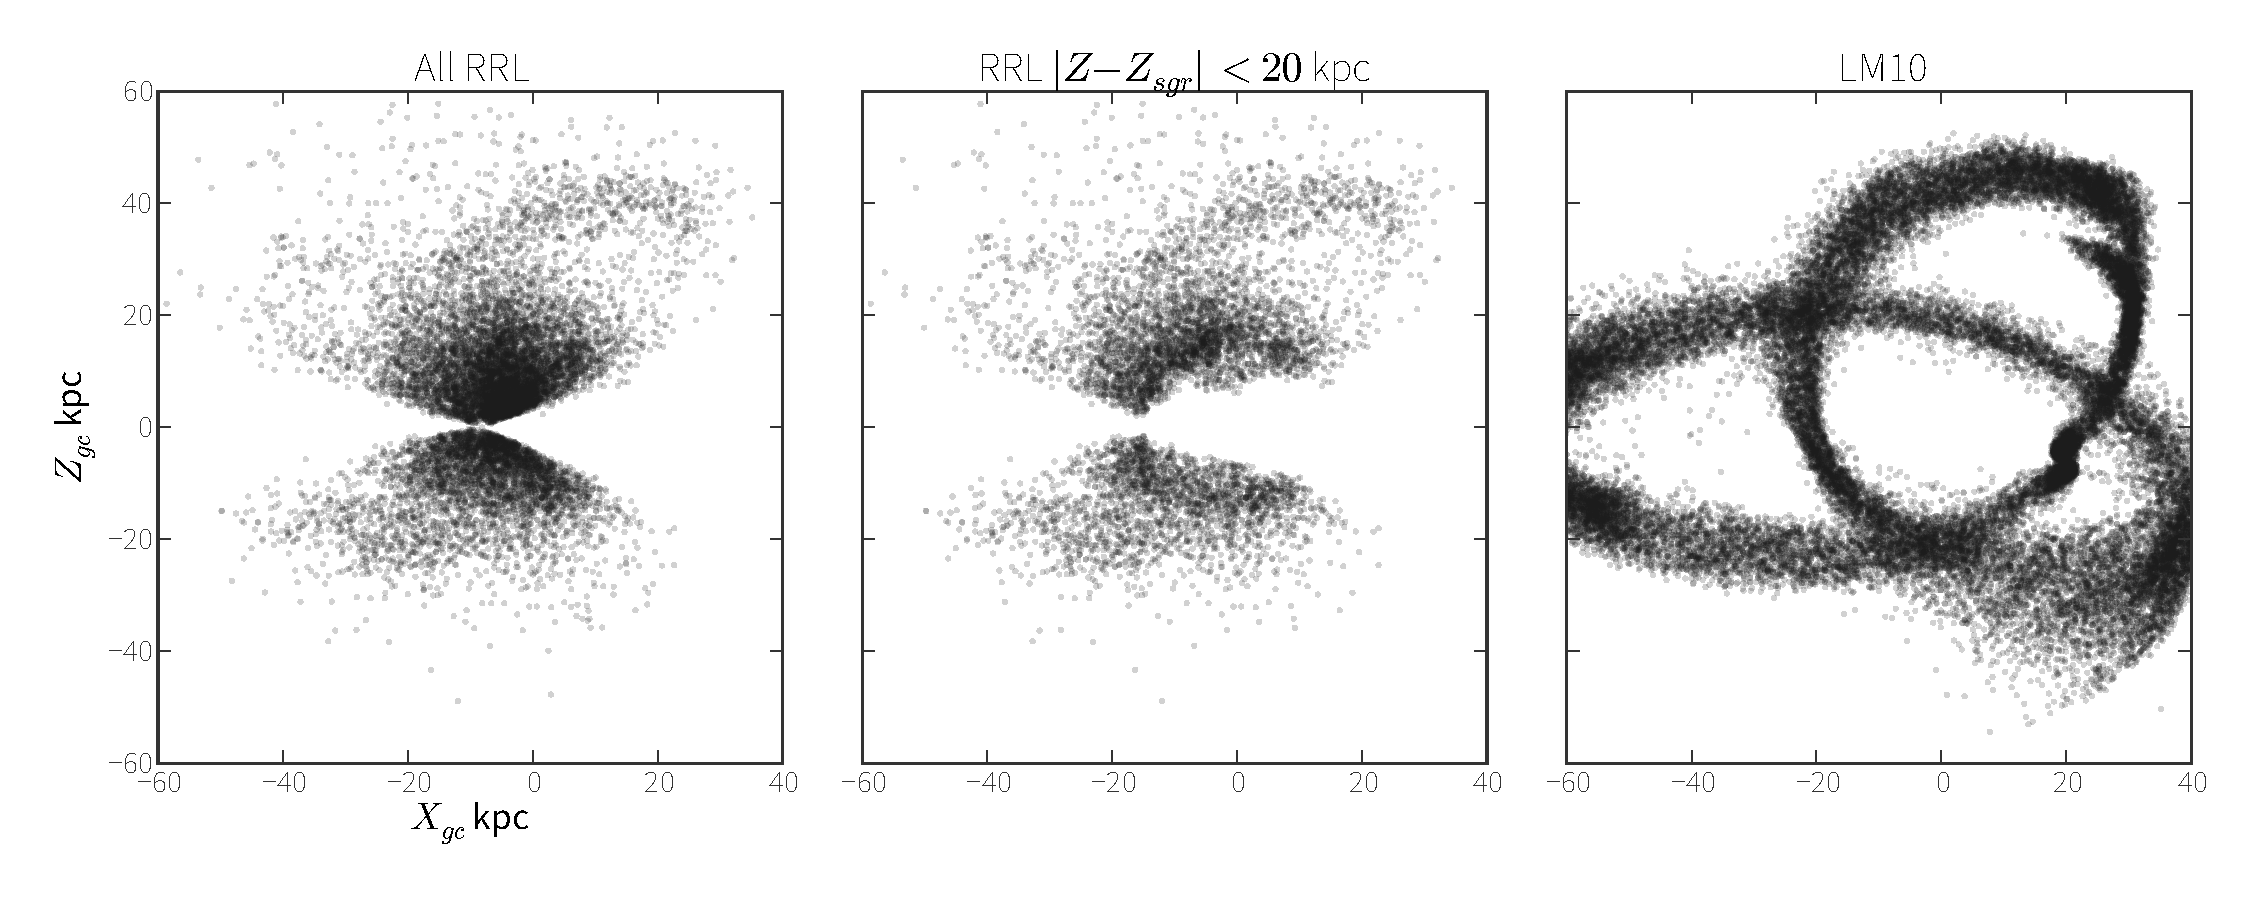
\includegraphics[width=0.9\textwidth]{catalina_all.pdf}
\caption{ From left to right: a) All CSS RRLs, b) CSS RRLs $<$ 20 kpc from the midplane of the Sgr coordinate system, and c) LM10 simulation particles. }\label{fig:css_all}
\end{center}
\end{figure}

\begin{figure}
\begin{center}
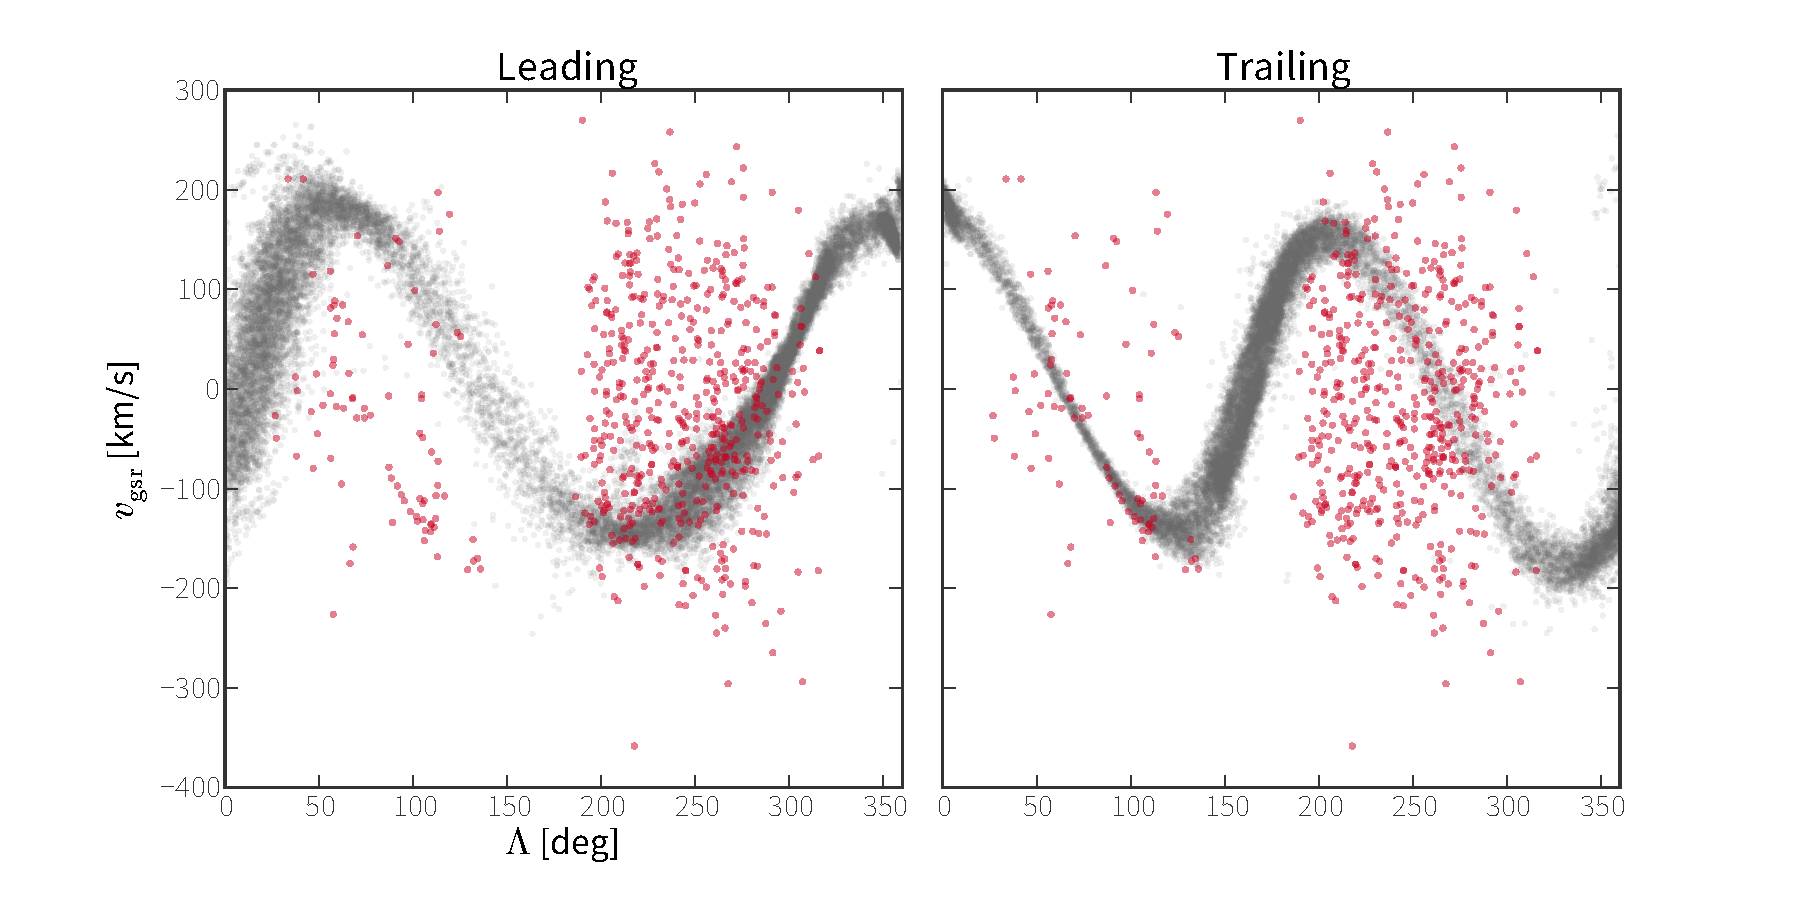
\includegraphics[width=0.75\textwidth]{catalina_all_vgsr.pdf}
\caption{ Galactocentric radial velocity for LM10 particles (grey) and CSS RRLs (red) for both the leading (left) and trailing (right) arms of Sgr debris. }\label{fig:css_vgsr}
\end{center}
\end{figure}

\begin{figure}
\begin{center}
\includegraphics[width=\textwidth]{dist_selection.pdf}
\caption{  CSS RRLs selected to be within $\pm$3-$\sigma$ from the median LM10 distance in each bin. }\label{fig:dist_selection}
\end{center}
\end{figure}

\begin{figure}
\begin{center}
\includegraphics[width=\textwidth]{vgsr_selection.pdf}
\caption{ CSS RRLs selected to be within $\pm$3-$\sigma$ from the median LM10 radial velocity in each bin. }\label{fig:vgsr_selection}
\end{center}
\end{figure}

\begin{figure}
\begin{center}
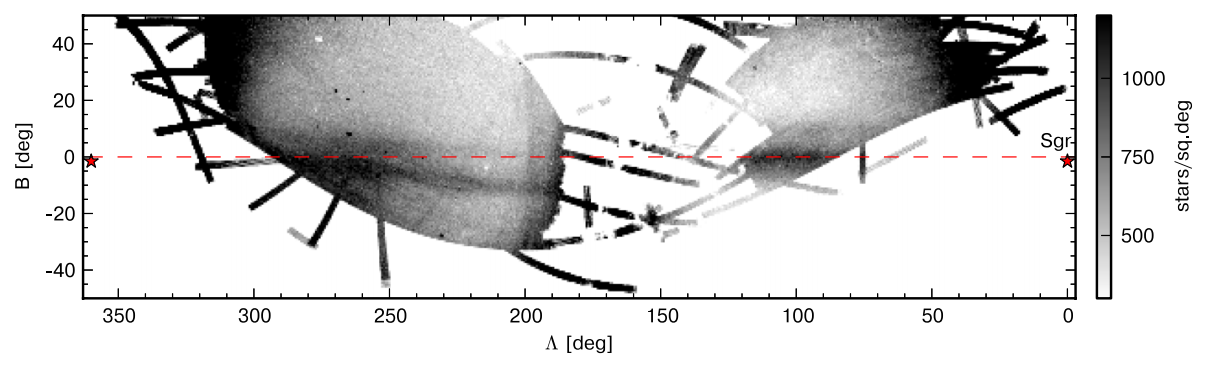
\includegraphics[width=\textwidth]{koposov.png}
\caption{ Figure~1 from Koposov et al. (2012), showing Sgr in the SDSS footprint. The bifurcation is near $B=0$ for $\Lambda>180$ and near $B=10$ for $\Lambda<180$. }\label{fig:koposov}
\end{center}
\end{figure}

\begin{figure}
\begin{center}
\includegraphics[width=\textwidth]{L_vs_B.pdf}
\caption{ $\Lambda$ vs. $B$ for LM10 particles (black) and selected particles (excluding the nearby trailing stars, for now). Blue are selected to not be associated with the bifurcation, green are the clump selected to be associated with the bifurcation. }\label{fig:LB}
\end{center}
\end{figure}


\begin{figure}
\begin{center}
\includegraphics[width=\textwidth]{with_near_trailing_xz.pdf}
\caption{ Final sample of CSS RRLs selected to be observed with Spitzer (green) and other RRLs that meet the criteria, but are unable to observe due to time constraints (red). }\label{fig:final_sample}
%Concentric circles with labels show required total integration time (over 12 visits) for a typical RR Lyrae at that distance.
\end{center}
\end{figure}

\end{document}
